\documentclass[aspectratio=169]{beamer}

\makeatletter
\defbeameroption{show only notes}[]% 
{
\beamer@notestrue
\beamer@notesnormalsfalse
}
\makeatother
\setbeameroption{hide notes}

%% ============ preamble
% !TEX root = ../digraph-main.tex
% packages.tex

% ----------------------------- Beamer Theme -----------------------------
\usetheme{Madrid}
\usepackage{appendixnumberbeamer}
\usefonttheme[onlymath]{serif}

% ----------------------------- Mathematics ------------------------------
\usepackage{amsmath}      % Advanced math formatting
\usepackage{amssymb}      % Additional math symbols
\usepackage{amsthm}       % Theorems and definitions
\usepackage{mathtools}    % Extensions to amsmath
\usepackage{bm}           % Bold math symbols
\usepackage{siunitx}      % SI units

% ----------------------------- Graphics ---------------------------------
\usepackage{graphicx}     % Include graphics
\usepackage{adjustbox}    % Adjust boxes, e.g., for resizing
\usepackage{tikz}         % Advanced graphics and drawing
\usetikzlibrary{
    arrows.meta,          % Arrow tips
    decorations.text,     % Text decorations
    automata, positioning, % Automata
    backgrounds,          % Background layers
    tikzmark,             % Markers for tikz
    calc                 % Calculations in tikz
}
\usepackage{animate}
\usepackage{media9}

% ----------------------------- Tables -----------------------------------
\usepackage{booktabs}     % Improved table formatting
\usepackage{multirow}     % Multirow cells
\usepackage{colortbl}     % Colored tables
\usepackage{tabularx}     % Tabular with flexible column widths
\usepackage{threeparttable} % Notes in tables
\usepackage{pdflscape}    % Landscape pages
\usepackage{float}

% ----------------------------- Algorithms ------------------------------
\usepackage[noend]{algorithm2e} % Algorithms with no end keywords
% \usepackage{algorithm}         % Algorithm package

% ----------------------------- Captions ---------------------------------
\usepackage[compatibility=false,
            justification=raggedright,
            font=scriptsize,
            singlelinecheck=true]{caption}
\usepackage[labelformat=empty,
            justification=raggedright]{subcaption}

% ----------------------------- Fonts ------------------------------------
\usepackage[T1]{fontenc}  % Font encoding
\usepackage[utf8]{inputenc} % UTF-8 input encoding
\usepackage{textcomp}     % Additional text symbols

% ----------------------------- Lists ------------------------------------
\usepackage{enumerate}    % Enhanced enumerate environment

% ----------------------------- References ------------------------------
\usepackage{cleveref}     % Smart cross-referencing
\crefname{proposition}{Proposition}{Propositions}
\Crefname{proposition}{Proposition}{Propositions}

% ----------------------------- Bibliography ----------------------------
\usepackage[hyperref=true,
            url=false,
            isbn=false,
            backref=false,
            doi=false,
            style=authoryear,
            uniquename=init,
            citereset=section,
            maxcitenames=1,
            maxbibnames=100,
            backend=bibtex,
            block=none]{biblatex}

% ----------------------------- Colors -----------------------------------
\usepackage{xcolor}       % Define and manage colors

% ----------------------------- Miscellaneous ---------------------------
\usepackage{hyperref}     % Hyperlinks in the document
\usepackage{tcolorbox}    % Colored boxes for emphasis
\usepackage{rotating}     % Rotating figures and tables
% !TEX root = ../digraph-main.tex
% customization.tex


\definecolor{applegreen}{rgb}{0.55, 0.71, 0.0}
\definecolor{dukeblue}{RGB}{0, 83, 155}
\definecolor{navyblue}{RGB}{1, 33, 105}

\setbeamercolor{frametitle}{bg=navyblue, fg=white}
% \setbeamertemplate{section in toc}[sections numbered]
% \setbeamertemplate{subsection in toc}[subsections numbered]
% \useoutertheme[subsection=false]{miniframes}
% \setbeamercolor{section in head/foot}{fg=white, bg=dukeblue}
% \setbeamerfont{section in head/foot}{series=\bfseries}

% \makeatletter
% \setbeamertemplate{frametitle}{%
%   \nointerlineskip%
%   \begin{beamercolorbox}[%
%       wd=\paperwidth,%
%       sep=0pt,%
%       leftskip=\metropolis@frametitle@padding,%
%       rightskip=\metropolis@frametitle@padding,%
%       ht=2.25ex,%%%%%% NEW !!!!!!!!!!!!!!!!!!!!!!!!!!!!!!!!!!!!!!!!
%       dp=1.1ex, %%%%%% NEW !!!!!!!!!!!!!!!!!!!!!!!!!!!!!!!!!!!!!!!!
%     ]{frametitle}%
%   \metropolis@frametitlestrut@start%
%   \insertframetitle%
%   \nolinebreak%
%   \metropolis@frametitlestrut@end%
%   \end{beamercolorbox}%
% }
% \makeatother

% get rid of navigation symbols
\setbeamertemplate{navigation symbols}{}

% remove shadow from title block
\setbeamertemplate{title page}[default][colsep=-4bp,rounded=true]

% use square-type bullets
\setbeamertemplate{itemize item}[circle]
\setbeamertemplate{itemize subitem}{--}
\setbeamertemplate{enumerate item}[circle]

% use circles for ToC items and correct the weird size issue with "Madrid" theme
\setbeamertemplate{sections/subsections in toc}[circle]
\setbeamerfont{section number projected}{size=\normalsize}

% figure captions: no "figure" prefix, small text, small figure-caption space
\captionsetup[figure]{labelformat=empty}
\captionsetup[table]{labelformat=empty}
\captionsetup[figure]{font=tiny,labelfont=tiny}
\captionsetup[subfigure]{font=tiny,labelfont=tiny}

% command for fixing inline TikZ nodes' vertical alignment
\newcommand{\tikzbasefix}{-\the\dimexpr\fontdimen22\textfont2\relax}

% define coloured clickable links
\hypersetup{%
  pdffitwindow=false,%
  pdfstartview={FitH},%
  % colorlinks,%
  pdfauthor={},%
  pdftitle={},%
  pagebackref=true,%
  citecolor=PaleGreen4,%
  filecolor=DarkOrchid4,%
  % linkcolor=OrangeRed4,%
  urlcolor=RoyalBlue4%
}

% define the includegraphics search path
\graphicspath{%
  {./figures/}%
}

% short-hand command for hyperlinked e-mails
\newcommand{\email}[1]{\href{mailto:#1}{\texttt{#1}}}

% customize TikZ matrix column separator character (to avoid Beamer
% conflict)
\tikzset{ampersand replacement=\&}

% redefine \boxed command to allow setting the border color
\newcommand{\highlight}[1]{\fcolorbox{complclr1}{white}{$\displaystyle #1$}}

% remove extra spacing around \left and \right delimiters
\let\leftorig\left
\let\rightorig\right
\renewcommand{\left}{\mathopen{}\mathclose\bgroup\leftorig}
\renewcommand{\right}{\aftergroup\egroup\rightorig}

% increase vertical spacing between table rows
\renewcommand{\arraystretch}{1.2}

% modified bullet-point for highlighting
\newcommand{\bulletemph}{$\large\boldsymbol{\star}$}

% superscript comma for footnote references
\newcommand{\footcomma}{\textsuperscript{,}}

% command to output names under images
\newcommand{\imentry}[3][1.25cm]{%
  \vbox{\halign{\hfil##\hfil\cr%
      \includegraphics[height=#1]{#2}\cr#3\cr}}}

% pictures goes with authors
\newcommand{\theauthor}[2]{\vbox{\halign{\hfil##\hfil\cr
  \includegraphics[width=0.125\textwidth]{#1}\cr#2\cr}}}

\newcommand{\theauthornopic}[1]{\vbox{\halign{\hfil##\hfil\cr
  \cr#1\cr}}}

\DeclareCaptionFont{tiny}{\tiny}

\newcommand{\backupbegin}{
   \newcounter{finalframe}
   \setcounter{finalframe}{\value{framenumber}}
}
\newcommand{\backupend}{
   \setcounter{framenumber}{\value{finalframe}}
}

\setbeamerfont{footnote}{size=\tiny}

% timeline option
\newlength\yearposx

% fix bug in beamer
% [https://tex.stackexchange.com/a/426090]
\makeatletter
\let\@@magyar@captionfix\relax
\makeatother

% alternative footnote by Tiancheng Liu
\newcommand\alternativefootnote[1]{%
 \tikz[remember picture,overlay]
 \draw (current page.south west) +(1in + \oddsidemargin,1em)
 node[anchor=south west,inner sep=0pt]{\parbox{\textwidth}{%
     \rlap{\rule{10em}{0.4pt}}\raggedright\tiny#1}};}


\def\signed #1{{\leavevmode\unskip\nobreak\hfil\penalty50\hskip1em
    \hbox{}\nobreak\hfill #1%
    \parfillskip=0pt \finalhyphendemerits=0 \endgraf}}

\newsavebox\mybox
\newenvironment{aquote}[1]
{\savebox\mybox{#1}\begin{quote}\hspace*{-.7ex}}
  {\unskip\vspace*{1mm}\signed{\usebox\mybox}\end{quote}}


% define new table columns for fixed-width center columns
% 
% [https://tex.stackexchange.com/a/12712]
\newcolumntype{C}[1]{>{\centering\let\newline\\\arraybackslash\hspace{0pt}}m{#1}}

% change how sections and subsection are highlight in TOC
\setbeamertemplate{section in toc}{
  \textbf{\inserttocsectionnumber.~\inserttocsection}}
\setbeamertemplate{section in toc shaded}{
  \inserttocsectionnumber.~\inserttocsection}

\setbeamertemplate{subsection in toc}{
  \hspace{1.2em}{\rule[0.3ex]{3pt}{3pt}}~\textbf{\inserttocsubsection}\par}
\setbeamertemplate{subsection in toc shaded}{
  \hspace{1.2em}{\rule[0.3ex]{3pt}{3pt}}~\inserttocsubsection\par}

% clever ref
\crefname{equation}{}{}
\Crefname{equation}{}{}

% extra rule for adding image with raggedright centered caption
\newcommand{\lcaption}[2]{ %
  % 
  \captionsetup{justification=raggedright}
  % 
  \begin{minipage}{#1}
    \caption{ %
      #2
    }
  \end{minipage}
}

\DeclareSIUnit{\nothing}{\relax}

\newcommand*{\textcal}[1]{%
  % family qzc: Font TeX Gyre Chorus (package tgchorus)
  % family pzc: Font Zapf Chancery (package chancery)
  \textbf{\textit{\fontfamily{qzc}\selectfont#1}}% 
}

\DeclareMathAlphabet{\zcal}{\encodingdefault}{sqzc}{m}{it}


\addtobeamertemplate{frametitle}{}{\vspace*{-0.5em}}


\newcommand{\gls}{G$\ell$S}

\newcommand{\conf}{\Omega}

\newcommand{\ha}{h_{\rm a}}
\newcommand{\hr}{h_{\rm r}}
\newcommand{\dm}{{{\em d.m.}}}

\newcommand{\bluered}{br}

\setbeamercolor{block body}{bg=dukeblue!30}
\setbeamercolor{block title}{bg=dukeblue,fg=black!2}


% theorem and collorary
\setbeamertemplate{theorems}[numbered] 

\makeatletter
\g@addto@macro\normalsize{%
    \setlength\abovedisplayskip{2pt}
}
\g@addto@macro\normalsize{%
    \setlength\belowdisplayskip{2pt}
}

\newcommand{\smsp}{\mspace{2mu}}  % slightly smaller space than \,
\DeclareMathOperator*{\argmax}{arg \smsp max}
\DeclareMathOperator*{\argmin}{arg \smsp min}

\newtheorem{proposition}{Proposition}


\def\arrowtext#1#2{\hbox to#1{\arrowtextA\ #2 \arrowtextA\kern2pt\llap{$\succ$}}}
\def\arrowtextA{\leaders\vrule height2.7pt depth-2.3pt\hfil}

\newcommand{\tikzvrule}[1]{
  \draw   ([yshift=-0.8cm,xshift=#1]current page.north west)
       -- ([xshift=#1]current page.south west)
}

\newcommand{\tikzvsubrule}[3]{
  \draw   ([yshift=-0.8cm+#2,xshift=#1]current page.north west)
       -- ([yshift=-0.8cm+#3,xshift=#1]current page.north west)
}

\newcommand{\tikzhrule}[1]{
  \draw   ([yshift=-0.8cm+#1]current page.north west)
       -- ([yshift=-0.8cm+#1]current page.north east)
}

\newcommand{\tikzhsubrule}[3]{
  \draw   ([yshift=-0.8cm+#1,xshift=#2]current page.north west)
       -- ([yshift=-0.8cm+#1,xshift=#3]current page.north east)
}


% footnote size & enable footnotes
% \renewcommand{\footnotesize}{\fontsize{5pt}{8pt}\selectfont}
% \let\oldfootnote\footnote
% \renewcommand\footnote[1][]{\oldfootnote[frame,#1]}

\renewcommand*{\bibfont}{\tiny}

% \AtEveryCitekey{
% %   \clearfield{location}
%   \clearfield{title}
%   \clearfield{number}
%   \clearfield{volume}
% %   \clearfield{publisher}
% }

\renewbibmacro*{cite}{%
  \iffieldundef{shorthand}
    {\ifthenelse{\ifnameundef{labelname}\OR\iffieldundef{labelyear}}
       {\usebibmacro{cite:label}%
        \setunit{\printdelim{nonameyeardelim}}}
       {\printnames{labelname}%
        \setunit{\printdelim{nameyeardelim}}}%
     \usebibmacro{cite:labeldate+extradate}%
     \setunit{\addcomma\space}%
     \usebibmacro{journal}}
   {\usebibmacro{cite:shorthand}}}

\setbeamertemplate{bibliography item}{}

%\makeatletter
%\newcommand{\xleftrightarrow}[2][]{\ext@arrow 3359\leftrightarrowfill@{#1}{#2}}
%\makeatother



% !TEX root = ../digraph-main.tex
% graphics.tex


% ---------- colors ---------- %

% color palette
\definecolor{baseclr}{HTML}{27408B}
\definecolor{myclr}{HTML}{000000}
\definecolor{complclr}{HTML}{CE9927}

% 2 complementary color sets
\definecolor{myblue}{HTML}{27408B}
\definecolor{myorange}{HTML}{CE9927}
\definecolor{myred}{HTML}{A92066}
\definecolor{mygreen}{HTML}{86BF24}

% alternative green-red combination
\definecolor{otherred}{HTML}{AA3939}
\definecolor{othergreen}{HTML}{2E882E}

% beamer colors
\setbeamercolor{normal text}{fg=baseclr}
\setbeamercolor{section in toc}{fg=baseclr}
\setbeamercolor{subsection in toc}{fg=baseclr}

% shade colors & listings

\definecolor{lightgray}{gray}{0.95} 
\definecolor{shadecolor}{rgb}{0.95,0.95,0.85}    % weights by xiaobai 

\sloppy


% !TEX root = ../digraph-main.tex
% extras.tex


\usetheme{Madrid}
\setbeamertemplate{caption}[numbered]
\setbeamertemplate{caption label separator}{: }
\setbeamercolor{caption name}{fg=normal text.fg}
\usepackage{lmodern}
\usepackage{amssymb,amsmath}
\usepackage{ifxetex,ifluatex}
\usepackage{fixltx2e} % provides \textsubscript
\ifnum 0\ifxetex 1\fi\ifluatex 1\fi=0 % if pdftex
  \usepackage[T1]{fontenc}
  \usepackage[utf8]{inputenc}
\else % if luatex or xelatex
  \ifxetex
    \usepackage{mathspec}
  \else
    \usepackage{fontspec}
  \fi
  \defaultfontfeatures{Mapping=tex-text,Scale=MatchLowercase}
  \newcommand{\euro}{€}
\fi
% use upquote if available, for straight quotes in verbatim environments
\IfFileExists{upquote.sty}{\usepackage{upquote}}{}
% use microtype if available
\IfFileExists{microtype.sty}{%
\usepackage{microtype}
\UseMicrotypeSet[protrusion]{basicmath} % disable protrusion for tt fonts
}{}
\usepackage{listings}
\usepackage{graphicx,grffile}
\makeatletter
\def\maxwidth{\ifdim\Gin@nat@width>\linewidth\linewidth\else\Gin@nat@width\fi}
\def\maxheight{\ifdim\Gin@nat@height>\textheight0.8\textheight\else\Gin@nat@height\fi}
\makeatother
% Scale images if necessary, so that they will not overflow the page
% margins by default, and it is still possible to overwrite the defaults
% using explicit options in \includegraphics[width, height, ...]{}
\setkeys{Gin}{width=\maxwidth,height=\maxheight,keepaspectratio}

% Comment these out if you don't want a slide with just the
% part/section/subsection/subsubsection title:
% \AtBeginPart{
%   \let\insertpartnumber\relax
%   \let\partname\relax
%   \frame{\partpage}
% }
%\AtBeginSection{
%  \let\insertsectionnumber\relax
%  \let\sectionname\relax
%  \frame{\sectionpage}
%}
%\AtBeginSubsection{
%  \let\insertsubsectionnumber\relax
%  \let\subsectionname\relax
%  \frame{\subsectionpage}
%}

% show plan before each section
\AtBeginSection[]
{
  \begin{frame}[noframenumbering,plain]
    % \frametitle{Outline}
    \tableofcontents[currentsection,
        currentsubsection,
        subsectionstyle=show/show/hide]
  \end{frame}
}

\setlength{\emergencystretch}{3em}  % prevent overfull lines
\providecommand{\tightlist}{%
  \setlength{\itemsep}{0pt}\setlength{\parskip}{0pt}}
\setcounter{secnumdepth}{0}

%% ============ set up the title slide and footer information

% title.tex
\title%
[ViT-RGTS]%  short version for footer
{A Study on ``Vision Transformers Need Registers''}%  long version

% -------------------- AUTHOR LIST ( & short info in FOOTER )
\author%
[Juntang Wang]% including photos and short info for FOOTER
{%
  Juntang Wang\footnotemark[1] 
  % \quad
  % Dongmian Zou\footnotemark[1]
}

\institute%
[DKU]% % short for FOOTER info
{%
  \inst{1}
  Duke Kunshan University (DKU), China%,
}

\date%
[\today]%
{\today}


% ========== bibliography
\bibliography{ref.bib}

\begin{document}

\frame{\titlepage}% the very first slide frame 

%%  ---------- Overview
%% ---frame 2
\begin{frame}
\frametitle{``Vision Transformers Need Registers'': Overview}

\cite{darcetVisionTransformersNeed2024}, \textit{ICLR}, Vision Transformers Need Registers

\vspace{1em}

\begin{itemize}
    \item \textbf{Paper Link:} \href{https://openreview.net/forum?id=2dnO3LLiJ1}{https://openreview.net/forum?id=2dnO3LLiJ1}
    \item \textbf{Repo. Link:} \href{https://github.com/kyegomez/Vit-RGTS}{https://github.com/kyegomez/Vit-RGTS} \quad (for replication)

    \vspace{1em}

    \item \textbf{TL;DR:}
    \begin{itemize}
        \item Vision Transformers (ViTs) exhibit \textbf{artifacts}: 
        $$\boxed{\text{high-norm tokens in low-information regions}}$$
        \item In both supervised and self-supervised; disrupt downstream tasks.
        \item \textbf{Registers}: additional tokens; only for internal computation.
        \item This approach:
        \begin{itemize}
            \item Achieves \textbf{SOTA} on dense prediction tasks.
            \item Enables \textbf{object discovery} in large models.
            \item Produces smoother \textbf{feature and attention maps}.
        \end{itemize}
    \end{itemize}
\end{itemize}
\end{frame}
%% ------------

%% ----------- Problems
\section{Problems}

\subsection{Motivation}

%% ---frame 3
\begin{frame}
\frametitle{Motivation}
\vspace{4.2em}
Big picture:

$$
\boxed{\text{Embedding images into generic features that can serve multiple purposes in CV}}
$$

\vspace{3.48em}

\begin{itemize}
        \item \textbf{Earlier, Handcrafted principles:} e.g., SIFT by Lowe 2004, IJCV.
        \item \textbf{Today, ``Labels are expensive''}:\textbf{Pretrain $\rightarrow$ feature extractor}
        \begin{itemize}
            \item For tasks with abundant data, pretrain a model.
            \item Use parts of the model as a feature extractor for downstream tasks.
        \end{itemize}
    \end{itemize}

\end{frame}
%% ------------

%% ---frame 4
\begin{frame}
\frametitle{Motivation (cont.)}
To bring us on the same page:

\begin{figure}[h]
    \centering
    \includegraphics[width=0.8\textwidth]{figures/attn6.png}
    \caption{Self-attention from a ViT trained with no supervision~(\cite{caronEmergingPropertiesSelfsupervised2021}).}
    \label{fig:attn6}
\end{figure}
\vspace{-1em}
\begin{itemize}
    \item Object segmentations from the self-attention\footnote{Self-attention of the \texttt{[CLS]} query produced by the last attention layer (\textbf{attention map}).}.
\end{itemize}

\end{frame}
%% ------------

%% ---frame 5
\begin{frame}
\frametitle{Motivation (cont.)}
\vspace{4.2em}
The paper's motivation:

$$
\boxed{\text{\emph{Observed: } In \underline{LOST}, DINOv2 \emph{worse} than DINO. } \quad \text{Analyze, fix these ViTs.}}
$$

\vspace{4.2em}
\underline{LOST\footnote{\cite{simeoniLocalizingObjectsSelfsupervised2021}, \textit{BMVC}; Seed points $\rightarrow$ full object regions.}}:
DINO features for Obj. detection\footnote{Not using attention maps (DINO-seg), but patch features.}.\quad $\rightarrow$ \quad $\boxed{\text{A clean attention map?}}$.
\end{frame}
%% ------------

%% ---frame 6
\begin{frame}
\frametitle{Motivation (cont.)}
\vspace{0.5em}
\begin{figure}[h]
    \centering
    {\footnotesize
    \setlength{\tabcolsep}{2.5pt} %
    \renewcommand{\arraystretch}{0.4} %
    \begin{tabular}{c cc cc cc }
      \vspace{0.2em}
      Input & DeiT-III-B & DeiT-III-L & OCLIP-B & OCLIP-L & DINO-B & DINOv2-g \\
      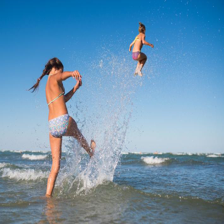
\includegraphics[width=0.10\textwidth]{resources/230914_1202_fig2_vizs_various_models/109_orig.png} &
      
\includegraphics[width=0.10\textwidth]{resources/230914_1202_fig2_vizs_various_models/deit3_base_patch16_224.fb_in22k_ft_in1k_109_lastattmap.png} &
      
\includegraphics[width=0.10\textwidth]{resources/230914_1202_fig2_vizs_various_models/deit3_large_patch16_224.fb_in22k_ft_in1k_109_lastattmap.png} &
      
\includegraphics[width=0.10\textwidth]{resources/230914_1202_fig2_vizs_various_models/vit_base_patch16_clip_224.laion2b_109_lastattmap.png} &
      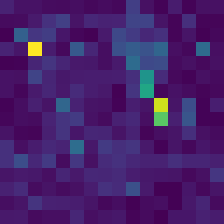
\includegraphics[width=0.10\textwidth]{resources/230914_1202_fig2_vizs_various_models/vit_large_patch14_clip_224.laion2b_109_lastattmap.png} &
      
\includegraphics[width=0.10\textwidth]{resources/230914_1202_fig2_vizs_various_models/vit_base_patch16_224.dino_109_lastattmap.png} &
      
\includegraphics[width=0.10\textwidth]{resources/230914_1202_fig2_vizs_various_models/vit_giant_patch14_dinov2.lvd142m_109_lastattmap.png}
      \\
      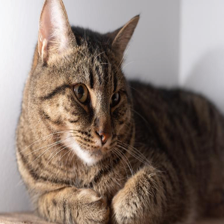
\includegraphics[width=0.10\textwidth]{resources/230914_1202_fig2_vizs_various_models/1500_orig.png} &
      
\includegraphics[width=0.10\textwidth]{resources/230914_1202_fig2_vizs_various_models/deit3_base_patch16_224.fb_in22k_ft_in1k_1500_lastattmap.png} &
      
\includegraphics[width=0.10\textwidth]{resources/230914_1202_fig2_vizs_various_models/deit3_large_patch16_224.fb_in22k_ft_in1k_1500_lastattmap.png} &
      
\includegraphics[width=0.10\textwidth]{resources/230914_1202_fig2_vizs_various_models/vit_base_patch16_clip_224.laion2b_1500_lastattmap.png} &
      
\includegraphics[width=0.10\textwidth]{resources/230914_1202_fig2_vizs_various_models/vit_large_patch14_clip_224.laion2b_1500_lastattmap.png} &
      
\includegraphics[width=0.10\textwidth]{resources/230914_1202_fig2_vizs_various_models/vit_base_patch16_224.dino_1500_lastattmap.png} &
      
\includegraphics[width=0.10\textwidth]{resources/230914_1202_fig2_vizs_various_models/vit_giant_patch14_dinov2.lvd142m_1500_lastattmap.png}
      \\
      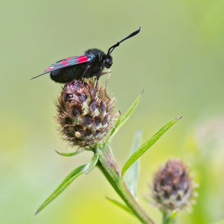
\includegraphics[width=0.10\textwidth]{resources/230914_1202_fig2_vizs_various_models/85_orig.png} &
      
\includegraphics[width=0.10\textwidth]{resources/230914_1202_fig2_vizs_various_models/deit3_base_patch16_224.fb_in22k_ft_in1k_85_lastattmap.png} &
      
\includegraphics[width=0.10\textwidth]{resources/230914_1202_fig2_vizs_various_models/deit3_large_patch16_224.fb_in22k_ft_in1k_85_lastattmap.png} &
      
\includegraphics[width=0.10\textwidth]{resources/230914_1202_fig2_vizs_various_models/vit_base_patch16_clip_224.laion2b_85_lastattmap.png} &
      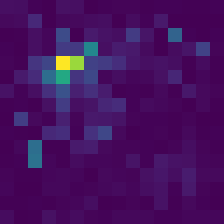
\includegraphics[width=0.10\textwidth]{resources/230914_1202_fig2_vizs_various_models/vit_large_patch14_clip_224.laion2b_85_lastattmap.png} &
      
\includegraphics[width=0.10\textwidth]{resources/230914_1202_fig2_vizs_various_models/vit_base_patch16_224.dino_85_lastattmap.png} &
      
\includegraphics[width=0.10\textwidth]{resources/230914_1202_fig2_vizs_various_models/vit_giant_patch14_dinov2.lvd142m_85_lastattmap.png}
      \\
      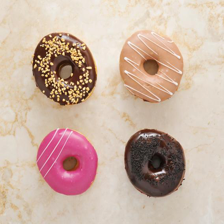
\includegraphics[width=0.10\textwidth]{resources/230914_1202_fig2_vizs_various_models/1753_orig.png} &
      
\includegraphics[width=0.10\textwidth]{resources/230914_1202_fig2_vizs_various_models/deit3_base_patch16_224.fb_in22k_ft_in1k_1753_lastattmap.png} &
      
\includegraphics[width=0.10\textwidth]{resources/230914_1202_fig2_vizs_various_models/deit3_large_patch16_224.fb_in22k_ft_in1k_1753_lastattmap.png} &
      
\includegraphics[width=0.10\textwidth]{resources/230914_1202_fig2_vizs_various_models/vit_base_patch16_clip_224.laion2b_1753_lastattmap.png} &
      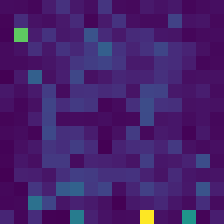
\includegraphics[width=0.10\textwidth]{resources/230914_1202_fig2_vizs_various_models/vit_large_patch14_clip_224.laion2b_1753_lastattmap.png} &
      
\includegraphics[width=0.10\textwidth]{resources/230914_1202_fig2_vizs_various_models/vit_base_patch16_224.dino_1753_lastattmap.png} &
      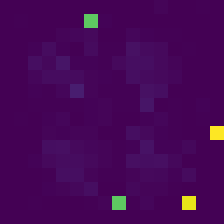
\includegraphics[width=0.10\textwidth]{resources/230914_1202_fig2_vizs_various_models/vit_giant_patch14_dinov2.lvd142m_1753_lastattmap.png}
      \\
    \end{tabular}
    }
    \vspace{-0.6em}
    \caption{
    %   We consider ViTs trained with label supervision (DeiT-III), text-supervision (OpenCLIP) or self-supervision (DINO and DINOv2).
      \emph{All models but DINO} exhibit $\boxed{\text{peaky outlier values}}$ in the attention maps~(\cite{darcetVisionTransformersNeed2024}).
    }  
    \label{fig:allvits}
\end{figure}
\end{frame}
%% ------------

%%

\subsection{Analysis}

%% ---frame 7
\begin{frame}
\frametitle{Analysis}

$$\boxed{\text{Artifacts are high-norm outlier tokens}}$$

\vspace{2em}
\begin{figure}[t]
    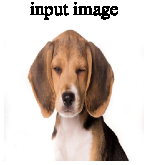
\includegraphics{resources/figure_3_1.pdf} 
    
\includegraphics{resources/figure_3_2.pdf} 
    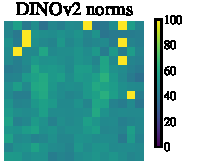
\includegraphics{resources/figure_3_3.pdf} 
    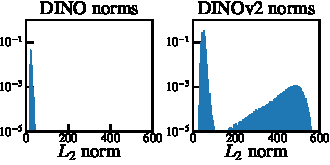
\includegraphics{resources/figure_3_4.pdf} 
    \caption{
      Comparison of local feature norms~(\cite{darcetVisionTransformersNeed2024})\footnote{150 is the threshold used for artifacts in the paper if not otherwise specified.}
    }  
    \label{fig:norms_hist}
\end{figure}
\end{frame}
%% ------------

%% ---frame 8
\begin{frame}
\frametitle{Analysis (cont.)}
\vspace{1em}

$$
\boxed{\text{Outliers appear during the training of large models}}
$$

\vspace{1em}
\begin{figure}[t]
    \centering
    \subcaptionbox{(a) Norms along layers.\label{fig:norm_hist_by_layer}}{
      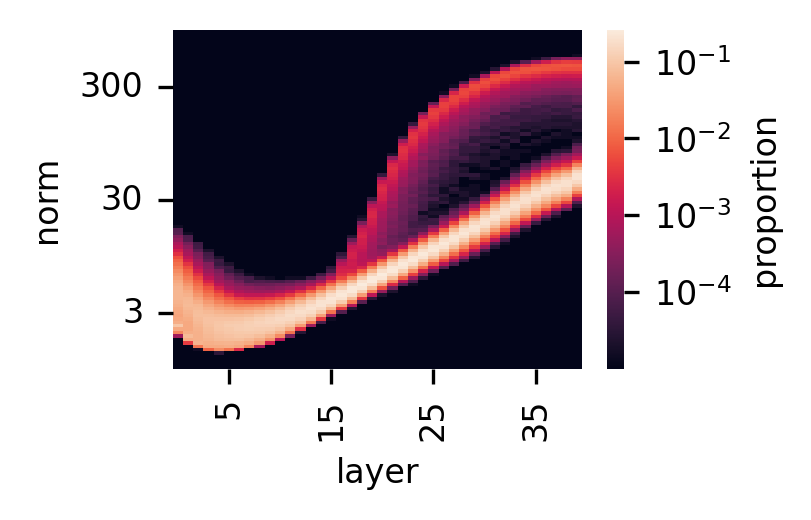
\includegraphics[width=0.31\linewidth]{resources/230802_norm_histogram_by_layer.png}
      \vspace{-1em}
    }
    \subcaptionbox{(b) Norms along iterations.\label{fig:norm_hist_by_iter}}{
      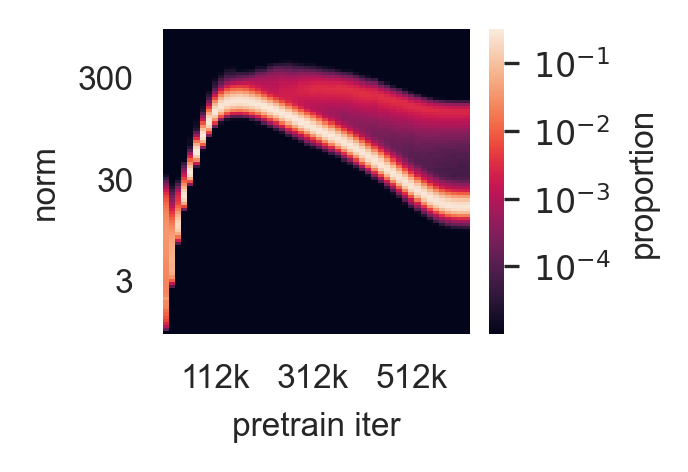
\includegraphics[width=0.31\linewidth]{resources/norm_distrib_vs_pretrain_iter.png}
      \vspace{-1em}
    }
    \subcaptionbox{(c) Norms across model size.\label{fig:norm_hist_by_model}}{
      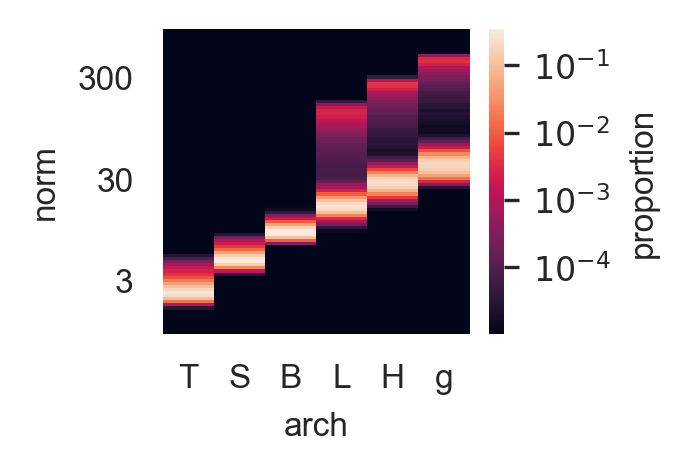
\includegraphics[width=0.31\linewidth]{resources/norm_distrib_vs_model_size.png}
      \vspace{-1em}
    }
    \vspace{-0.648em}
    \caption{
        Illustration of several properties of outlier tokens~(\cite{darcetVisionTransformersNeed2024})\footnote{40-layer DINOv2 ViT-g model.}.
    }
    \label{fig:factors_choice}
\end{figure}
\end{frame}
%% ------------

%% ---frame 9
\begin{frame}
\frametitle{Analysis (cont.)}
\vspace{1em}

$$
\boxed{\text{High-norm tokens appear where patch information is redundant (Fig.~\ref{fig:outlier_cos_sims})}}
$$

\vspace{1em}
\begin{figure}[t]
    \centering
    \subcaptionbox{(a) Cosine similarity to neighbors.\label{fig:outlier_cos_sims}}{
      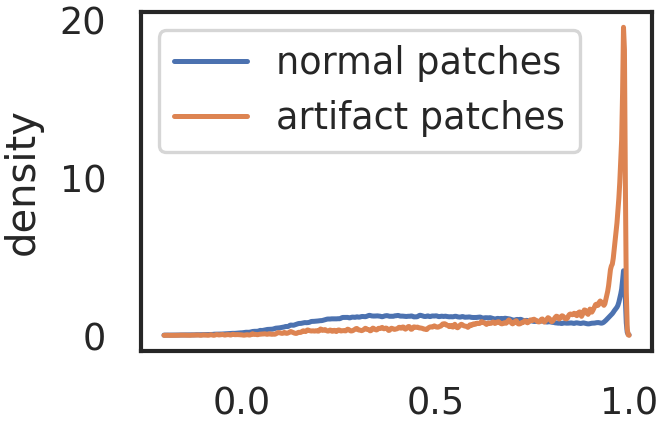
\includegraphics[width=0.3\linewidth]{resources/230802_kde_cossim_neighbors_2.png}
    }
    \hfill
    \subcaptionbox{(b) Linear probing for local information.\label{tab:logreg_weird_patches_local}}{
      \begin{tabular}{@{} l c cc c c @{}}
        \toprule
                && \multicolumn{2}{c}{position prediction} && reconstruction\\
        \cmidrule{3-4} \cmidrule{6-6}
                && top-1 acc      & avg. distance $\downarrow$ && L2 error $\downarrow$\\
        \midrule
        normal  && \textbf{41.7}  & \textbf{0.79} && \textbf{18.38} \\
        outlier && 22.8           & 5.09          && 25.23 \\
        \bottomrule
      \end{tabular}
    }
    \caption{
      (a): Distribution of cosine similarity between input patches and their 4 neighbors.
      (b): Local information probing on normal and outlier patch tokens~(\cite{darcetVisionTransformersNeed2024}).
    }
\end{figure}
\end{frame}
%% ------------

%% ---frame 10
\begin{frame}
\frametitle{Analysis (cont.)}

$$
\boxed{\text{High-norm tokens hold little local information (Tab.~\ref{tab:logreg_weird_patches_local})}}
$$

$$
\boxed{\text{Artifacts hold global information (Tab.~\ref{tab:logreg_weird_patches_image_classif})}}
$$

\begin{table}[t]
    \centering
    \caption{%
        Image classification via linear probing on normal and outlier patch tokens~(\cite{darcetVisionTransformersNeed2024})\footnote{Also report the accuracy of classifiers learnt on the class token.}.
      }
    \vspace{-1em}
    \begin{tabular}{@{} l *{14}{c@{\hspace{4pt}}} @{}}
      \toprule
      & IN1k & P205 & Airc. & CF10 & CF100 & CUB & Cal101 & Cars & DTD & Flow. & Food & Pets & SUN & VOC \\
      \midrule
      \texttt{[\texttt{[CLS]}]} & \textbf{86.0} & \textbf{66.4} & \textbf{87.3} & \textbf{99.4} & \textbf{94.5} & \textbf{91.3} & \underline{96.9} & \textbf{91.5} & \textbf{85.2} & \textbf{99.7} & \textbf{94.7} & \textbf{96.9} & \textbf{78.6} & \underline{89.1} \\
      normal & 65.8 & 53.1 & 17.1 & 97.1 & 81.3 & 18.6 & 73.2 & 10.8 & 63.1 & 59.5 & 74.2 & 47.8 & 37.7 & 70.8 \\
      outlier & \underline{69.0} & \underline{55.1} & \underline{79.1} & \underline{99.3} & \underline{93.7} & \underline{84.9} & \textbf{97.6} & \underline{85.2} & \underline{84.9} & \underline{99.6} & \underline{93.5} & \underline{94.1} & \underline{78.5} & \textbf{89.7} \\
      \bottomrule
    \end{tabular}
    \vspace{-1em}
    \label{tab:logreg_weird_patches_image_classif}
\end{table}

\end{frame}
%% ------------

%%

%%%

%% ----------- Methods
\section{Method}

\subsection{Hypothesis}

%% ---frame 11
\begin{frame}
\frametitle{Hypothesis}
In ViT
\begin{itemize}
    \item Large, long iterations $\rightarrow$ artifacts.
    \item \emph{Artifacts are not inherently bad} \footnote{They often appear in low-information regions and their local role can be recovered by surrounding tokens.}.
    \item However, LOST suffers \footnote{And other tasks that rely on \emph{clean local features}.}.
\end{itemize}
\end{frame}
%% ------------

%% ---frame 12
\begin{frame}
\frametitle{Hypothesis (cont.)}
Inspired by \cite{bulatovRecurrentMemoryTransformer2022}, add \emph{registers} tokens\footnote{First proposed for remediate translation in NLP.}:

$$
\boxed{\text{Additional learnable input tokens, discarded in output.}}
$$

\vspace{1em}
This should isolate the global context, preserving clean, local patch features.
\end{frame}
%% ------------

%%

\subsection{Remediation}
%% ---frame 13
\begin{frame}
\frametitle{Remediation}
\begin{figure}[t]
    \centering
    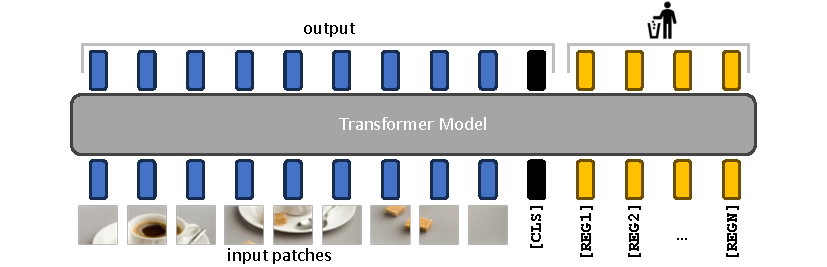
\includegraphics{resources/model.pdf} 
    \caption{
      Illustration of the proposed remediation and resulting model.~(\cite{darcetVisionTransformersNeed2024}).
    }  
    \vspace{-1em}
    \label{fig:model}
  \end{figure}
\end{frame}
%% ------------

%%

%%%

%% ----------- Results
\section{Experiments}

%% ---frame 14
\begin{frame}
\frametitle{Experimental Setup}
\vspace{2.3em}
\begin{table}[h]
    \centering
    \caption{Summary of models used in this paper's experiments.}
    \begin{tabular}{lllll}
        \toprule
        Method & Sup. & Dataset & Arch. & Paper \\
        \midrule
        DEIT-III \footnote{\url{https://github.com/facebookresearch/deit}} & Label & ImageNet-22k & ViT-B & \cite{touvronDeiTIIIRevenge2022} \\
        OpenCLIP \footnote{\url{https://github.com/mlfoundations/open_clip}} & Text & Shutterstock & ViT-B/16 & \cite{ilharco_gabriel_2021_5143773} \\
        DINOv2 \footnote{\url{https://github.com/facebookresearch/dinov2}} & Self & ImageNet-22k & ViT-L & \cite{oquabDINOv2LearningRobust2024} \\
        \bottomrule
    \end{tabular}
    \label{tab:methods}
\end{table}
\end{frame}
%% ------------

\subsection{Evaluation}

%% ---frame 15
\begin{frame}
\frametitle{Evaluation}
\vspace{2em}

$$
\boxed{\text{Register tokens effectively remove the norm outliers that were present previously.}}
$$

\vspace{2em}
\begin{figure}[t]
    \centering
    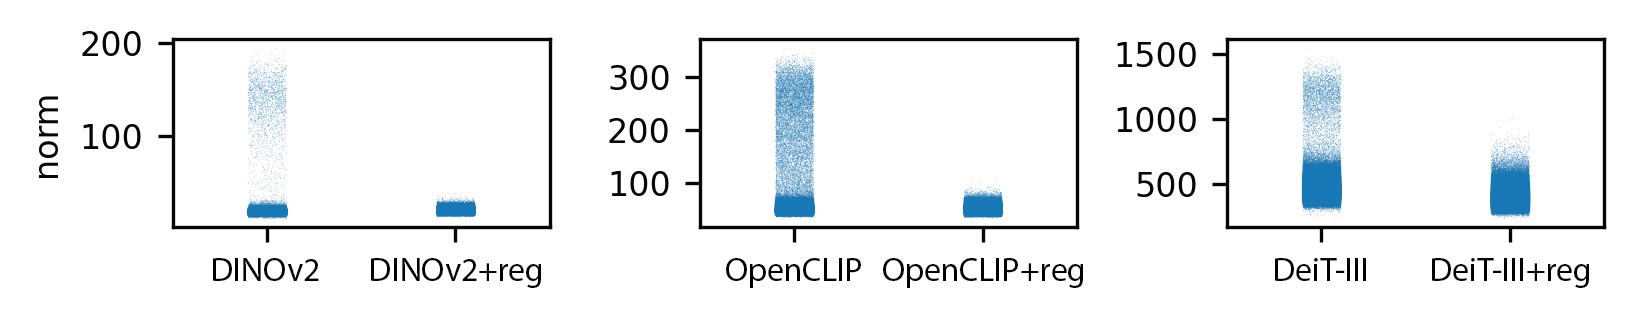
\includegraphics[width=\textwidth]{resources/fig_norm_distrib_before_after_stripplot-2.png}
    \caption{
      Effect of register tokens on the distribution of output norms~(\cite{darcetVisionTransformersNeed2024}).
    }
    \label{fig:norm_distrib_before_after}
\end{figure}

\end{frame}
%% ------------

%% ---frame 16
\begin{frame}
\frametitle{Evaluation (cont.)}

Using registers not only \emph{does not degrade performance}, but even:

$$
\boxed{\text{improves performance by a slight margin in some cases (Tab.~\ref{tab:downstream})}}
$$

\end{frame}
%% ------------

    




%% ---frame 17
\begin{frame}
\frametitle{Evaluation (cont.)}

\begin{table}[h]
    \centering
    \caption{
        Evaluation of downstream performance of the models that we trained, with and without registers.
      }  
    \subcaptionbox{(a) Linear evaluation with frozen features.\label{tab:linear}}{
      \centering
      \begin{tabular}{@{}l c ccc@{}}
          \toprule
                      & ImageNet & ADE20k  & NYUd \\
                      & Top-1  & mIoU    & rmse $\downarrow$ \\
          \midrule
        DeiT-III      & 84.7   & 38.9   & 0.511    \\
        DeiT-III+reg  & 84.7   & 39.1   & 0.512    \\
        \midrule
        OpenCLIP      & 78.2   & 26.6   & 0.702    \\
        OpenCLIP+reg  & 78.1   & 26.7   & 0.661    \\
        \midrule
        DINOv2        & 84.3 & 46.6 & 0.378 \\
        DINOv2+reg    & 84.8 & 47.9 & 0.366 \\
          \bottomrule
      \end{tabular}
    }
    \hspace{3em}
    \subcaptionbox{(b) Zero-shot classification.\label{tab:zero-shot}}{
      \begin{tabular}{@{}l c c@{}}
          \toprule
                      & ImageNet \\
                      & Top-1  \\
          \midrule
        OpenCLIP      & 59.9    \\
        OpenCLIP+reg  & 60.1    \\
          \bottomrule
      \end{tabular}
    }
    \label{tab:downstream}
\end{table}

\end{frame}
%% ------------

%%

\subsection{Ablation study}

%% ---frame 18
\begin{frame}
\frametitle{Ablation study}

To remove artifacts\footnote{Evaluated on three tasks (ImageNet, ADE-20k and NYUd)}::

$$
\boxed{\text{One register is sufficient, more leads to improved downstream performance. (Fig.~\ref{fig:scores_n_reg})}}
$$

\end{frame}
%% ------------

%% ---frame 19
\begin{frame}
\frametitle{Ablation study (cont.)}
\begin{figure}[t]
    \centering
    \begin{tabular}{*{7}{>{\centering\arraybackslash}m{0.135\textwidth}@{}}}
      Input & 0 \texttt{[reg]} & 1 \texttt{[reg]} & 2 \texttt{[reg]} & 4 \texttt{[reg]} & 8 \texttt{[reg]} & 16 \texttt{[reg]} \\
      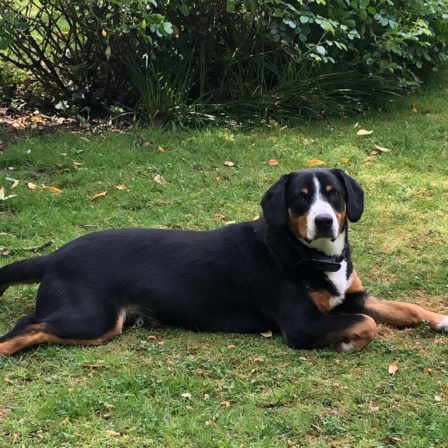
\includegraphics[width=0.13\textwidth]{resources/230916_attmap_vs_n_reg/pyrrhus_orig.png} &
      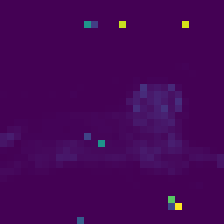
\includegraphics[width=0.13\textwidth]{resources/230916_attmap_vs_n_reg/100cc_pyrrhus_0reg.png} &
      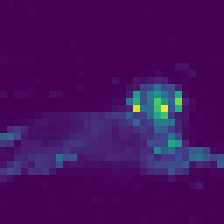
\includegraphics[width=0.13\textwidth]{resources/230916_attmap_vs_n_reg/100cc_pyrrhus_1reg.png} &
      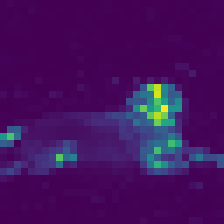
\includegraphics[width=0.13\textwidth]{resources/230916_attmap_vs_n_reg/100cc_pyrrhus_2reg.png} &
      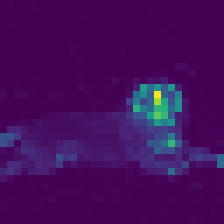
\includegraphics[width=0.13\textwidth]{resources/230916_attmap_vs_n_reg/100cc_pyrrhus_4reg.png} &
      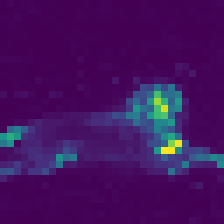
\includegraphics[width=0.13\textwidth]{resources/230916_attmap_vs_n_reg/100cc_pyrrhus_8reg.png} &
      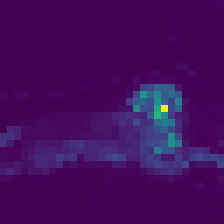
\includegraphics[width=0.13\textwidth]{resources/230916_attmap_vs_n_reg/100cc_pyrrhus_16reg.png}
    \end{tabular} \\
    \vspace{0.3em}
    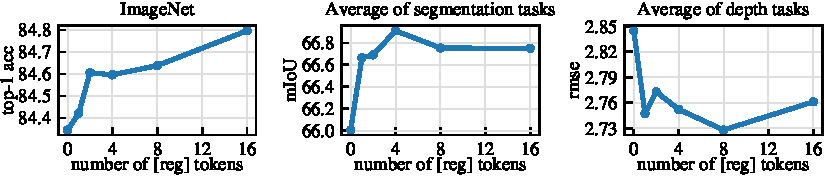
\includegraphics{resources/ablation_n_reg.pdf}
    \caption{
      Ablation of the the number of register tokens used with a DINOv2 model~(\cite{darcetVisionTransformersNeed2024}).
    }
    \label{fig:scores_n_reg}
\end{figure}
\end{frame}
%% ------------

%%

\subsection{Other experiments}

%% ---frame 20
\begin{frame}
\frametitle{Other experiments - Object discovery}

$$
\boxed{\text{Registers \emph{significantly} improve object discovery performance (Tab.~\ref{tab:lost})}}
$$

\begin{table}[t]
    \centering
    \begin{tabular}{@{}l c ccc@{}}
        \toprule
                    & VOC 2007 & VOC 2012  & COCO 20k \\
        \midrule
      DeiT-III      & 11.7 & 13.1 & 10.7 \\
      DeiT-III+reg  & 27.1 & 32.7 & 25.1 \\
      \midrule
      OpenCLIP      & 38.8 & 44.3 & 31.0 \\
      OpenCLIP+reg  & 37.1 & 42.0 & 27.9 \\
      \midrule
      DINOv2        & 35.3 & 40.2 & 26.9 \\
      DINOv2+reg    & 55.4 & 60.0 & 42.0 \\
        \bottomrule
    \end{tabular}
    \caption{
      Unsupervised Object Discovery using LOST on models with and without registers~(\cite{darcetVisionTransformersNeed2024})\footnote{Performance measured using corloc.}.
    %   We observe that adding register tokens makes all models significantly more viable for usage in object discovery.
    }  
    \label{tab:lost}
\end{table}
\end{frame}
%% ------------

%% ---frame 21
\begin{frame}
\frametitle{Other experiments - Qualitative evaluation}

Similarly to slot attention~(\cite{locatelloObjectCentricLearningSlot2020})\footnote{This behaviour was never required from the model, and emerged naturally from training.}:

$$
\boxed{\text{Register tokens attend to different parts of the feature map.}}
$$

{\footnotesize
(It's a pity that this behaviour is not explored further in the paper.)
}

\begin{figure}[t]
    \begin{tabular}{cccccc}
      Input & \texttt{[\texttt{[CLS]}]} & \texttt{[reg$_0$]} & \texttt{[reg$_6$]} & \texttt{[reg$_8$]} & \texttt{[reg$_{12}$]} \\
      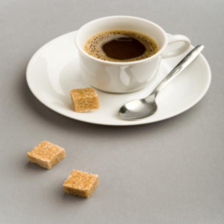
\includegraphics[width=0.13\textwidth]{resources/230913_fig_slot_attn/mug.png} &
      \includegraphics[width=0.13\textwidth]{resources/230913_fig_slot_attn/mug_attn_cls.png} &
      \includegraphics[width=0.13\textwidth]{resources/230913_fig_slot_attn/mug_attn_reg_0.png} &
      \includegraphics[width=0.13\textwidth]{resources/230913_fig_slot_attn/mug_attn_reg_6.png} &
      \includegraphics[width=0.13\textwidth]{resources/230913_fig_slot_attn/mug_attn_reg_8.png} &
      \includegraphics[width=0.13\textwidth]{resources/230913_fig_slot_attn/mug_attn_reg_12.png}
      \\
    \end{tabular}
    \caption{
      Comparison of the attention maps of the \texttt{[CLS]} and register tokens~(\cite{darcetVisionTransformersNeed2024}).
    }
    \label{fig:slot_attn}
\end{figure}

\end{frame}
%% ------------

%%

%%%

%% ----------- Discussion
\section{Conclusion}

%% ---frame 22
\begin{frame}
\frametitle{Conclusion}
\begin{itemize}
    \item \emph{Artifacts}.
    \item — likely due to iterations and larger model.
    \item A possible interpretation: the model reuse low-info areas to store \emph{global context}.
    \item \emph{Artifacts are not inherently bad}, but can hurt LOST\footnote{And other tasks that rely on clean feature maps}.
    \item \emph{Register tokens} act as a decoupling mechanism.
    \item Different register tokens seem to focus on \emph{different objects}.
\end{itemize}
\end{frame}
%% ------------

%%

\section{Further work}

%% ---frame 23
\begin{frame}
\frametitle{Further work}

\begin{itemize}
    \item \emph{One more benchmark}. Object discovery $[\text{TBD}]$
    \begin{itemize}
        \item \emph{Open Images, Object365}, WIDER FACE, DeepFashion2, KITTI, AIOD
    \end{itemize}
    \item \emph{Improve the model / one more benchmark}:
\end{itemize}
\begin{figure}[t]
    \centering
    \caption{
        Preliminary results of our study.
    }
    \subcaptionbox{(a) Linear evaluation with frozen features.}{
        \centering
        \begin{tabular}{@{}l c@{}}
            \toprule
                            & Tiny ImageNet\footnote{\url{https://paperswithcode.com/dataset/tiny-imagenet}} \\
                            & Top-1  \\
            \midrule
          DeiT-B/16-D       & 91.0   \\
          DeiT-B/16-D+reg   & 90.8   \\
            \bottomrule

        \end{tabular}
      }
    \subcaptionbox{(b) Zero-Shot Classification.}{
        \begin{tabular}{@{}l c c@{}}
            \toprule
                                & ImageNet \\
                                & Top-1  \\
            \midrule
          OC(ResNet50)          & 59.6    \\
          OC(ResNet50)+reg      & 60.0    \\
          OC(ViT-B/32)          & 63.2    \\
          OC(ViT-B/32)+reg      & 61.4    \\
            \bottomrule
        \end{tabular}
      }
\end{figure}

\end{frame}

%% ---frame 24
\begin{frame}
\frametitle{Further work (cont.)}

\begin{itemize}
    \item Different registers may attend to different objects — test this more directly.
    \begin{itemize}
        \item CLEVR, COCO Panoptic, GQA
    \end{itemize}
    \item \emph{Move beyond ViT}. e.g. Sequence data, matrix data. Reached T10 on a recent Kaggle\footnote{\url{https://www.kaggle.com/competitions/stanford-rna-3d-folding}}
    \item \emph{Move beyond ViT}. e.g. Configurations from Multi-Resolution Graph-based Clustering\footnote{\url{https://www.qqgjyx.com/mheatmap/}}
\end{itemize}
\vspace{-2em}
\begin{figure}[t]
    \centering
    \includegraphics[width=\textwidth]{figures/cifar10_attnmap.png}
\end{figure}
\end{frame}
%% ------------

%%

%%%

%% -----------  Acknowledgement

\section*{Acknowledgement}
% !TEX root = ../digraph-main.tex

\begin{frame}{Acknowledgements}

  \begin{columns}
    \begin{column}{0.35\textwidth}
      We thank xxx for xxx 
    \end{column}
    \hspace*{2em}
    \begin{column}{0.45\textwidth}
      This work is supported in part by
      \begin{list}{$\diamond$}{\itemsep = 3pt \leftmargin=10pt}
        \item research grant xxxx
        \item research grant xxxx 
      \end{list}
    \end{column}
  \end{columns}

\end{frame}



%% ============ BIBLIOGRAPHY
\section*{Bibliography}
\appendix

\begin{frame}[noframenumbering,plain,allowframebreaks]{References}
    \printbibliography[heading=none]
\end{frame}


\end{document}


%%%%

%%%%  provided by Xiaobai Sun 
%%%%
